\section{Simuladores de realidad virtual}
\label{art:simulador}

\begin{figure}[h]
   \centering
    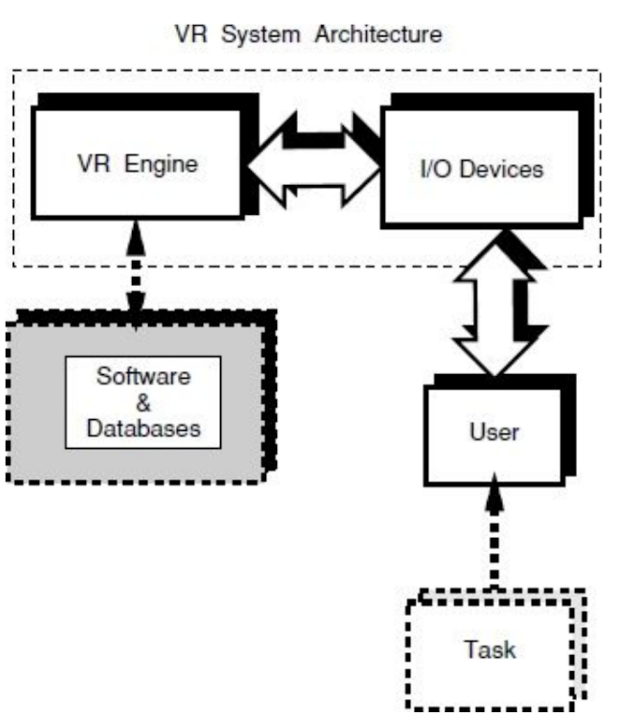
\includegraphics[width=0.5\textwidth]{IMG/VRarq.PNG}
    \caption{Arquitectura propuesta por \cite{burdea2003virtual} }
   \label{fig:RVarq}
\end{figure}
Según \emph{Burdea y Coiffet}\cite{burdea2003virtual}, un sistema de \ac{RV} se puede dividir en cinco componentes como se puede observar en la figura \ref{fig:RVarq}. En ella podemos observar las distintas interacciones que se producen entre componentes. De manera separada, estos componentes pueden existir independientemente pero es la relación entre ellos la que componen un sistema \ac{RV}. A continuación se describirá cada uno de ellos:
\begin{itemize}
    \item Motor de \ac{RV}: Este componente se encarga de realizar los cálculos necesarios para simular la escena virtual. Para actualizar el estado de la escena virtual, es necesario que consulte las bases de datos y software incluidos en el sistema y actuará según la entrada recibida a través de los dispositivos realizada por los usuarios. El motor generará y mostrará el nuevo estado de la escena a través de los dispositivos de salida (que pueden incluir más de un canal sensorial). Además, es preciso asegurar una tasa interactiva al realizar estos cálculos. Este término se tiene que tratar como una abstracción ya que puede tener múltiples configuraciones hardware como puede ser un computador o un sistema distribuido conectado por red.
    \item Dispositivos de \ac{E/S}: Este componente se basa en todos los dispositivos que utilice el usuario en su interacción con el sistema. Es imprescindible en un sistema \ac{RV} permita la interacción del usuario. Los dispositivos de entrada se encargan de recoger las acciones que realiza el usuario, y recibe la respuesta de la escena virtual a través de los dispositivos de salida de los distintos canales sensoriales. Estos dispositivos son muy numerosos y diversos actualmente.
    \item Componentes software y base de datos: Este módulo contiene todas las especificaciones y descripciones que caracterizan el sistema y la escena virtual. Aquí se incluyen la escena virtual y su organización que es consultada por el motor de \ac{RV} análogamente a lo que correspondería como una base de datos, donde se consulta y se recoge la información necesaria para la simulación. Además, aquí se incluyen, por ejemplo, las aplicaciones que se diseñan con el objetivo de guiar y facilitar el entrenamiento al dirigir la simulación según la interacción del sistema y el usuario.
    \item Usuario: Es natural que los sistemas se diseñen con el objetivo de que una persona interaccionará y espera una respuesta en forma de estímulos a través de los dispositivos de \ac{E/S}. 
    \item Tareas: Por último, son las tareas, objetivos e instrucciones que se le dan al usuario cuando va a utilizar el sistema \ac{RV} que le dan significado y utilidad al simulador. Es lo que le diferencia de ser un computador con periféricos conectados de una plataforma de entrenamiento para pilotos o médicos. 
    
\end{itemize}

Esta definición de arquitectura será utilizada en el capítulo \ref{cap:rasim} como apoyo para explicar el simulador \ac{RASim} y sus diferentes componentes. A su vez, también puede ayudar al lector a hacerse una idea de como se 





\subsection{Simuladores para formación médica}
\label{art:medicalsim}

En los últimos años, los simuladores médicos de realidad virtual están tomando una gran importancia en el currículum de los estudiantes, como pueden ser los cirujanos y otras especialidades \cite{PATEL2017266.e7}. Se puede observar un incremento de su presencia para el entrenamiento de jóvenes especialistas tanto en hospitales como universidades. Estas herramientas proporcionan al usuario un método seguro y efectivo de entrenamiento, siendo capaces de usarlo tantas veces como sea posible. 

Aun con la introducción de los simuladores, todavía el entrenamiento médico se basa en una variedad de técnicas que permite al médico adquirir las destrezas necesarias antes de poder enfrentarse a escenarios reales de manera autónoma. Una forma segura de entrenamiento es la utilización de \emph{fantomas}\cite{phantomra}. En la figura \ref{fig:phantom} se puede ver un maniquí \emph{Blue Phantom™}\cite{BluePH}.

\begin{figure}[h]
   \centering
    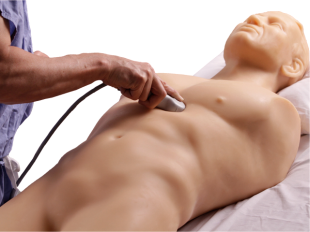
\includegraphics[width=0.5\textwidth]{IMG/fast_trauma.jpg}
    \caption{Maniquí realista para el entrenamiento de ultrasonidos \emph{Blue Phantom™}\cite{BluePH} }
   \label{fig:phantom}
\end{figure}

Estos \emph{fantomas}\footnote{castellanización del término inglés Phantom} son modelos anatómicos hechos con materiales sintéticos intentando replicar el cuerpo humano fielmente y sus propiedades. En ocasiones, tienen incorporados una serie de sensores que permiten recogida de métricas. A pesar de que son muy populares, tiene una serie de inconvenientes: no son baratos, y suelen ser creados específicamente para una zona anatómica concreta, no siendo posible usarlos en otras circunstancias para lo que fueron creados. Además, si en determinadas ocasiones, el usuario tiene que manipularlos como puede ser hacer una incisión o inyección en el \emph{fantoma}, el modelo sufre desgaste con el tiempo.

Otra forma de entrenamiento es la utilización de cadáveres\cite{Tsui2007}, que permiten una anatomía real muy alejada de los muñecos poco realistas. En este caso, conseguir diferentes variaciones anatómicas es completamente viable y el mismo cadáver puede servir para entrenamientos de diferentes procedimientos. Aun así, los inconvenientes que presentan son bastante evidentes. Mantener un cadáver en buenas condiciones y que los motivos del fallecimiento perjudiquen al estado del mismo, son los principales problemas que nos encontramos además de ciertos problemas éticos como puede ser el uso de cadáveres procedentes de condenados a pena de muerte como puede ser el Visible Human Project \cite{ackerman1998visible}. Introducir sensores o algún tipo de dispositivo que permitan evaluar el rendimiento tampoco es sencillo. Finalmente, los tejidos de un cadáver no muestran el mismo comportamiento mecánico que un paciente, y puede inducir sesgos en el entrenamiento del médico debido a que los músculos se vuelven más rígidos después del fallecimiento.


La última forma de entrenamiento es el entrenamiento sobre pacientes reales, donde al estudiante realiza el procedimiento supervisado y guiado por su tutor. Aunque es el entrenamiento más realista, obviamente incluye una serie de riesgos y situaciones no controladas que pueden ser peligrosas para el paciente.


A diferencia de los métodos anteriormente citados, los simuladores de realidad virtual permiten un entrenamiento más barato y rápido donde los estudiantes pueden mejorar sus habilidades. Mejoras en el rendimiento, nuevos dispositivos periféricos y desarrollo de nuevas técnicas de simulación física permiten una transferencia efectiva de habilidades del mundo virtual al mundo real, como podemos observar a continuación.
Habitualmente los simuladores  son específicos de cada procedimiento médico donde podemos encontrar un simulador de cirugía ortopédica \cite{cecil2017advanced}, o por ejemplo un simulador de cirugía cardiovascular \cite{korzeniowski2018vcsim3}. Incluso, podemos incluir diferentes tipos de simulación, donde \cite{villard2014interventional} es un simulador de radiología intervencional donde además de entrenar la habilidad manual, es necesario aprender como guiar la aguja a través de imagen de rayos X.

Pero además, la nueva generación de simuladores no solo se centran en mejorar la calidad de la simulación, sino que también quieren permitir el entrenamiento con datos de pacientes reales\cite{Willaert2012,  Votta2013}. 






\subsection{Diagnóstico por imagen médica}
\label{art:xraysim}

En radiología, la forma más común de aprender diagnóstico por imagen son los archivos educativos. Son recopilaciones de imágenes médicas de pacientes reales acompañados normalmente del historial del paciente. En estos archivos, los estudiantes pueden buscar a través de la gran cantidad de casos bien documentados. Normalmente, cada universidad, hospital o facultad tienen sus propios repositorios, incluso existen libros que se pueden consultar como \cite{carver2012medical}.
En la última década, cada vez más se publican estos recursos de manera online donde cualquier radiólogo pueda consultar un enorme base de datos de imágenes de cualquier parte de la anatomía humana \cite{deshpande2017integrated}. 

Actualmente, la educación se ha visto beneficiada por la incorporación de los teléfonos inteligentes en este ámbito. Algunas instituciones han creado aplicaciones donde los estudiantes pueden revisar e investigar los casos almacenados, realizar cuestionarios y mejorar el aprendizaje como es el caso de la aplicación \emph{UBC Radiology} \cite{Spouge2017}. Estos recursos se encuentran muy presentes en el aprendizaje de los radiólogos noveles, pero todos estos recursos mantienen el mismo problema. Las imágenes registradas son estáticas, y la mayoría de estas imágenes corresponden a imágenes que se presuponen que son correctas y no muestran ningún tipo de fallo. Esto es completamente entendible, ya que al hacer este tipo de recursos se seleccionan para intentar ser educativos. Además, ninguna imagen es del mismo paciente en diferentes situaciones o partes del cuerpo por razones de seguridad. Aun así, posicionar bien al paciente mientras se realiza el diagnóstico por imagen es algo imprescindible y algo necesario que el estudiante domine.

Mejoras en el rendimiento de los computadores permiten crear nuevos simuladores que mejoran y reducen el tiempo de aprendizaje de los estudiantes. Un caso remarcable es el  ProjectionVR$^{TM}$ \cite{shanahan2016student}. Este simulador trata de introducir al usuario dentro de un entorno realista 3D que quiere replicar una sala de rayos X para simular el procedimiento completo. Con datos de pacientes reales digitalizados, el simulador replica un entorno de aprendizaje sin el consecuente riesgo de radiación que significaría exponer a los estudiantes o los pacientes. Aunque provee una cantidad amplia de datos médicos, los datos que contienen son estáticos y los usuarios no pueden variarla o modificarla en el simulador. 

%https://www.bluephantom.com/product/Sciatic-Nerve-Regional-Anesthesia-Ultrasound-Training-Model.aspx?cid=428


\subsection{Anestesia regional}

Como se ha comentado con la anterior sección, existen multitud de simuladores dependiendo de su procedimiento médico que se pretende simular. En cuanto a la especialidad de anestesiología, la anestesia espinal y la epidural son los dos ejemplos más frecuentes dentro de la anestesia regional y podemos encontrar simuladores específicos \cite{broom2018evaluation}. Sin embargo, la búsqueda de un simulador de anestesia regional genérico es más complicada. Energid Technologies ha desarrollado  un simulador en un contrato con el Ejército de Estados Unidos, pero no ha sido comercializado al público \cite{lim2008simulation}.

Otro simulador, en este caso comercial, llamado SAILOR es distribuido acompañado de un atlas multimedia de los bloqueos de nervios. Este simulador presenta solo un único modelo de paciente, y su interacción es exclusivamente con el ratón sin ninguna tipo de deformación del tejido. \cite{Bibin}

En un estudio previo al proyecto RASimAs, se demostró la aceptación que tendría un simulador para la anestesia regional. Todos los participantes se mostraron muy receptivos con el trabajo realizado, sin embargo, se pudo constatar la escasez de nervios para bloquear, la pobre simulación de los ultrasonidos y una respuesta háptica realista \cite{Grottke2009594}.

%https://www.gtsimulators.com/Full-Body-X-Ray-Phantom-with-Real-Human-Skeleton-p/ez7200.htm